\section{Results} \label{sec:results}
Some general stuff here

\subsection{Determine the energy in the Ising model}
We have determined the energy of the Ising model using both linear regression (OLS, Ridge and Lasso) and neural networks, where we first train the model on a set, and then validate the model on a test set. In project 1, we found our implementation of OLS, Ridge and Lasso to give the same result as Scikit Learn, and we will in this project stick to Scikit Learn due to its quickness. [Ref. project 1] Let's start with linear regression. 

\subsubsection{Linear regression}
We used linear regression to find the $\bb{J}$-matrix, and from that we found the energies. In table \eqref{tab:lin_reg}, the errors between obtained energy and true energy are listed for the training set, the test set and the K-fold cross-validation resampling. Further, the $\bb{J}$-matrix is visualized in figure \eqref{fig:J_matrix} and the R$^2$-score is plotted as function of $\lambda$ in figure \eqref{fig:lambda_vs_R2_linear}.

\begin{table} [H]
	\caption{Mean Square Error and R$^2$-score presented for OLS, Ridge and Lasso on the Ising model. 'Train' means the results obtained from the training set, containing 8000 states, and 'Test' means the results obtained from the test set, containing 2000 states. The 'K-fold'-columns are results from K-fold resampling with 10 folds. For Ridge and Lasso, we used $\lambda=1e-3$ (penalty). See text for more information.}
	\begin{tabularx}{\textwidth}{l|XXX|XXX} \hline\hline
		\label{tab:lin_reg}
		& \multicolumn{3}{c}{\textbf{MSE}}&\multicolumn{3}{c}{\textbf{R2}}\\ \hline
		&Train&Test&K-fold&Train&Test&K-fold\\ \hline
		OLS & 0.3006 & 0.3006 & 0.3739 & 0.9925 & 0.9927 & 0.9906\\
		Ridge & 1.731e-13 & 2.150-13 & 1.618e-13 & 1.000 & 1.000 & 1.000 \\
		Lasso & 4.029e-5 & 4.189e-5 & 4.0346e-5 & 1.000 & 1.000 & 1.000 \\ \hline\hline
	\end{tabularx}
\end{table}

We observe that the MSE is quite low, especially for Ridge and Lasso. The R$^2$-score is correspondingly high. Below, in figure \eqref{fig:J_matrix}, the $\bb{J}$-matrix is visualized for all the linear regression methods and $\lambda\in[1e-1,1e-6]$.

\newgeometry{left=2cm,right=2cm,top=2cm}
\begin{figure} [H]%
	\centering
	\subfloat[OLS, $\lambda=0.1$]{{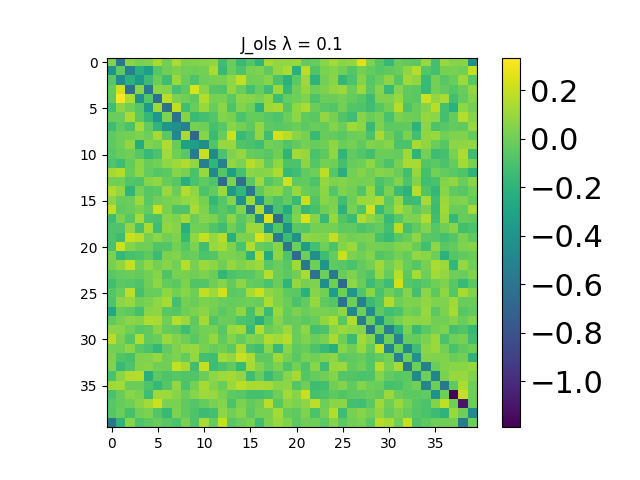
\includegraphics[width=6cm]{../plots/J_ols_lambda_1.png}}}
	\subfloat[Ridge, $\lambda=0.1$]{{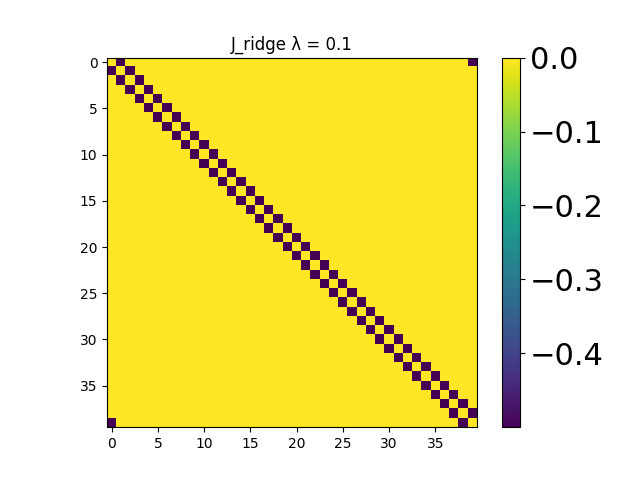
\includegraphics[width=6cm]{../plots/J_ridge_lambda_1.png} }}
	\subfloat[Lasso, $\lambda=0.1$]{{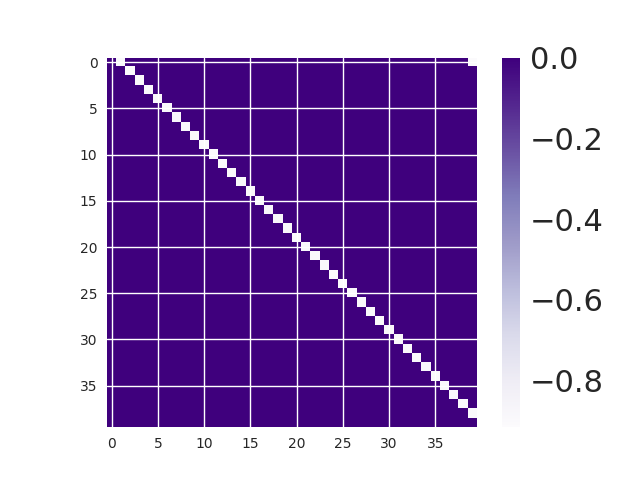
\includegraphics[width=6cm]{../plots/J_lasso_lambda_1.png} }}\\
	
	\subfloat[OLS, $\lambda=0.001$]{{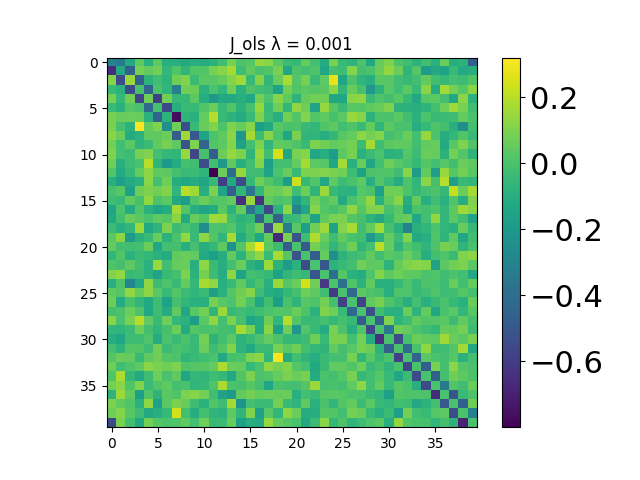
\includegraphics[width=6cm]{../plots/J_ols_lambda_3.png} }}%
	\subfloat[Ridge, $\lambda=0.001$]{{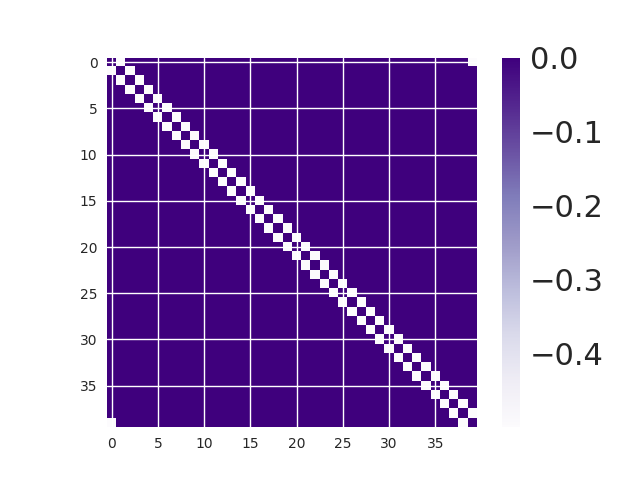
\includegraphics[width=6cm]{../plots/J_ridge_lambda_3.png} }}
	\subfloat[Lasso, $\lambda=0.001$]{{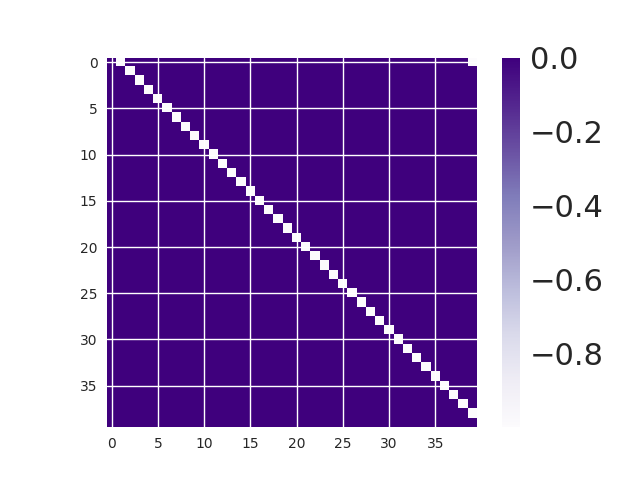
\includegraphics[width=6cm]{../plots/J_lasso_lambda_3.png} }}\\
	
	\subfloat[OLS, $\lambda=0.0001$]{{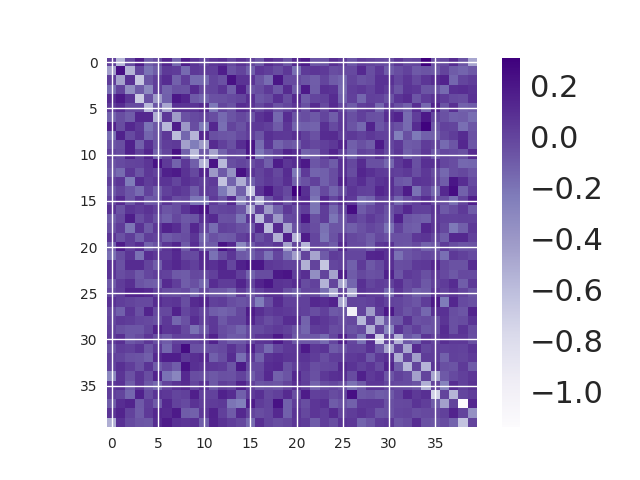
\includegraphics[width=6cm]{../plots/J_ols_lambda_4.png} }}%
	\subfloat[Ridge, $\lambda=0.0001$]{{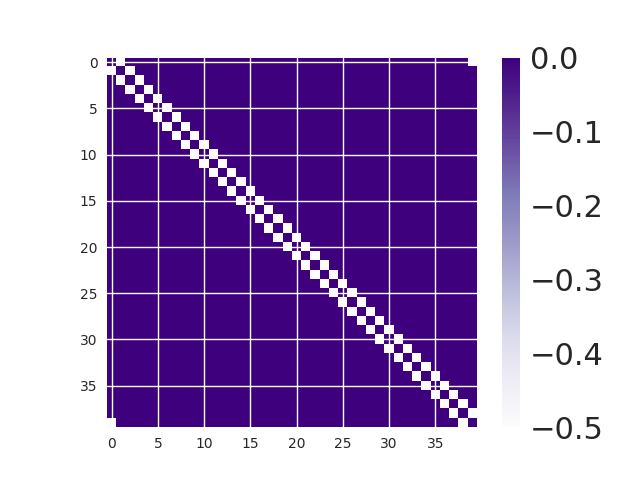
\includegraphics[width=6cm]{../plots/J_ridge_lambda_4.png} }}
	\subfloat[Lasso, $\lambda=0.0001$]{{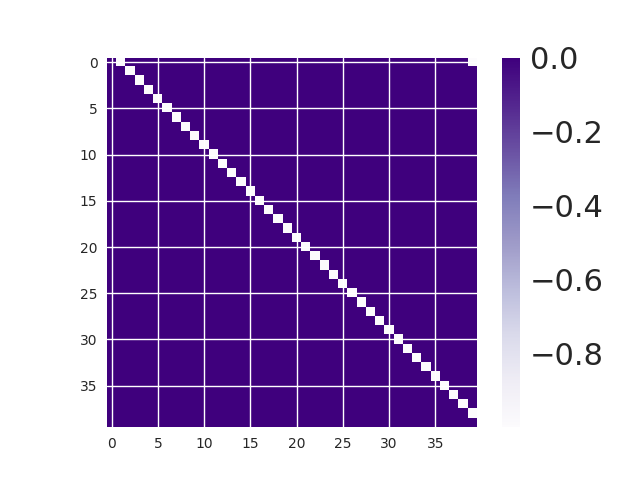
\includegraphics[width=6cm]{../plots/J_lasso_lambda_4.png} }}\\
	
	\subfloat[OLS, $\lambda=0.000001$]{{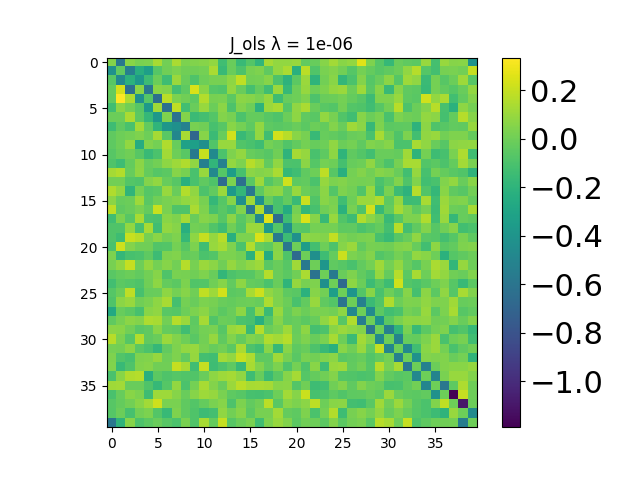
\includegraphics[width=6cm]{../plots/J_ols_lambda_6.png} }}%
	\subfloat[Ridge, $\lambda=0.000001$]{{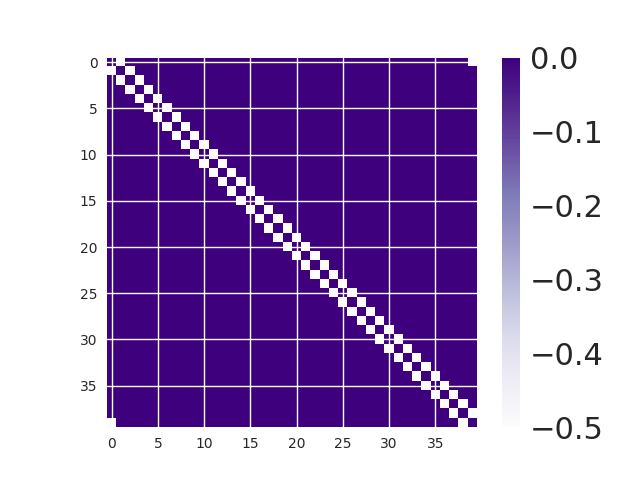
\includegraphics[width=6cm]{../plots/J_ridge_lambda_6.png} }}
	\subfloat[Lasso, $\lambda=0.000001$]{{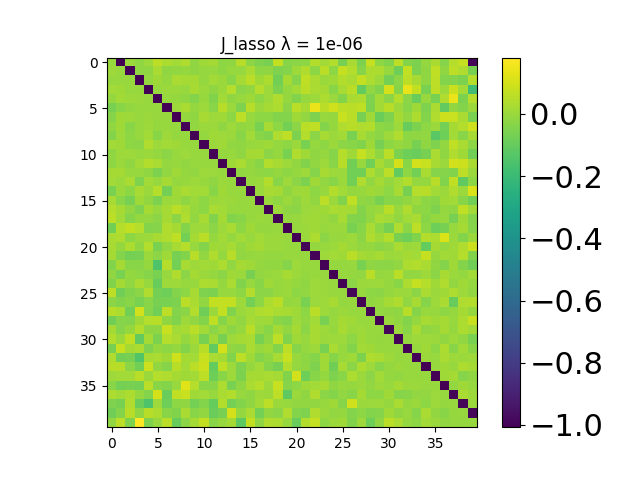
\includegraphics[width=6cm]{../plots/J_lasso_lambda_6.png} }}
	\caption{The J-matrix obtained from OLS, Ridge and Lasso with $\lambda\in[1e-1,1e-6]$. The models where trained on 8000 randomly chosen Ising states.}%
	\label{fig:J_matrix}
\end{figure}
\restoregeometry
We observe that the $\bb{J}$ obtained form Lasso is superdiagonal, while for Ridge it is sub-superdiagonal. For OLS, the matrix tends to be sub-superdiagonal, but the off-diagonal elements are not fully zero. 

Finally, the R$^2$-score is plotted as a function of the penalty, $\lambda$, in figure \eqref{fig:lambda_vs_R2_linear}.
\iffalse
\begin{figure} [H]
	\centering
	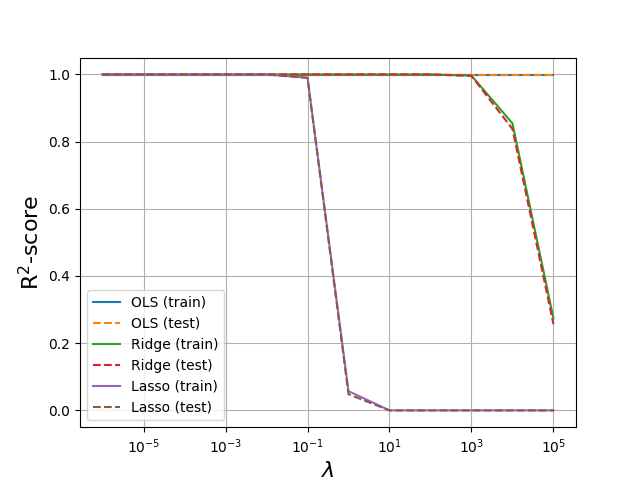
\includegraphics[scale=0.65]{../plots/lambda_vs_R2_linear.png}
	\caption{The R$^2$-score as a function of the penalty. }
	\label{fig:lambda_vs_R2_linear}
\end{figure} 
\fi

\subsubsection{Neural networks}
We now repeat what we have done above, jump over to a neural network approach. 
\begin{table} [H]
	\caption{Mean Square Error and R$^2$-score presented for OLS, Ridge and Lasso on the Ising model. 'Train' means the results obtained from the training set, containing 8000 states, and 'Test' means the results obtained from the test set, containing 2000 states. The 'K-fold'-columns are results from K-fold resampling with 10 folds. For Ridge and Lasso, we used $\lambda=1e-3$ (penalty). See text for more information.}
	\begin{tabularx}{\textwidth}{l|XXX|XXX} \hline\hline
		\label{tab:nn}
		& \multicolumn{3}{c}{\textbf{MSE}}&\multicolumn{3}{c}{\textbf{R2}}\\ \hline
		Hidden nodes&Train&Test&K-fold&Train&Test&K-fold\\ \hline
		0 & 3.529e-4 & 4.454e-4 & 3.610e-4 & 1.000 & 1.000 & 1.000\\
		2 & 0.009128 & 0.009651 & 0.009128 & 0.8977 \\
		5 & 0.01439 & 0.01489 & 0.01555 & 0.8387 \\
		10 & 0.01439 & 0.01489 & 0.01555 & 0.8387 \\
		2 + 2 & 0.01439 & 0.01489 & 0.01555 & 0.8387 \\
		5 + 5 & 0.01439 & 0.01489 & 0.01555 & 0.8387 \\ 
		10 + 10 & 0.01439 & 0.01489 & 0.01555 & 0.8387 \\
		10 + 10 + 10 & 0.01439 & 0.01489 & 0.01555 & 0.8387 \\ \hline\hline
	\end{tabularx}
\end{table}

\subsection{Classifying the phase}
Removed states around critical temperature.

\subsubsection{Logistic regression}
\begin{table} [H]
	\caption{Accuracy score}
	\begin{tabularx}{\textwidth}{l|XX|XX} \hline\hline
		\label{tab:logistic_regression}
		& \multicolumn{2}{c}{\textbf{GD}}&\multicolumn{2}{c}{\textbf{SGD}}\\ \hline
		Iterations&Train&Test&Train&Test\\ \hline
		10 & 3.529e-4 & 4.454e-4 & 3.610e-4 & 1.\\
		100 & 0.009128 & 0.009651 & 0.009128 & 0.8977 \\
		1000 & 0.01439 & 0.01489 & 0.01555 & 0.8387 \\ \hline\hline
	\end{tabularx}
\end{table}

Add lambda as accuracy score plot

\subsubsection{Neural networks}






